\documentclass[conference]{IEEEtran}
\IEEEoverridecommandlockouts

\usepackage{cite}
\usepackage{amsmath,amssymb,amsfonts}
\usepackage{mathtools}
\usepackage{algorithmic}
\usepackage{graphicx}
\usepackage{textcomp}
\usepackage{xcolor}
\usepackage{textcomp}
\usepackage{float}
\usepackage{array}
\usepackage{siunitx}
\usepackage{tabularx}
\usepackage{listings}
\usepackage[colorlinks=false]{hyperref}
\def\BibTeX{{\rm B\kern-.05em{\sc i\kern-.025em b}\kern-.08em
    T\kern-.1667em\lower.7ex\hbox{E}\kern-.125emX}}

\setlength{\parindent}{0pt}

% Define the custom column type Y
\newcolumntype{Y}{>{\centering\arraybackslash} m{1.1cm}}

\definecolor{codeblue}{rgb}{0.2,0.2,0.6}
\definecolor{codegreen}{rgb}{0.133,0.545,0.133}
\definecolor{codegray}{rgb}{0.5,0.5,0.5}
\definecolor{codepurple}{rgb}{0.58,0,0.82}
\definecolor{backcolour}{rgb}{0.95,0.95,0.92}

\lstdefinestyle{mystyle}{
    backgroundcolor=\color{backcolour},
    commentstyle=\color{codegreen},
    keywordstyle=\color{codeblue},
    numberstyle=\tiny\color{codegray},
    stringstyle=\color{codepurple},
    basicstyle=\ttfamily\scriptsize,
    breakatwhitespace=false,
    breaklines=true,
    captionpos=b,
    keepspaces=true,
    numbers=none,
    numbersep=5pt,
    showspaces=false,
    showstringspaces=false,
    showtabs=false,
    tabsize=2
}

\lstset{style=mystyle}

\begin{document}

\title{Robotics and Mechatronics\\
{\LARGE Homework Two}
}

\author{\IEEEauthorblockN{Mohammad Montazeri}
    \IEEEauthorblockA{\textit{School of Mechanical Engineering} \\
        \textit{College of Engineering, University of Tehran}\\
        Tehran, Iran; 810699269 \\
        mohammadmontazeri@ut.ac.ir}
}

\maketitle

\begin{abstract}
    This homework mainly focuses on analyzing serial robots and modeling them based on Denavit-Hartenberg theories. Overall, four examples of important and widely used robotic arms are discussed in terms of their forward and inverse kinematics problems. Also, software modeling is implemented for one of these problems using MATLAB to verify the analytical results.
\end{abstract}

\begin{IEEEkeywords}
    forward kinematics problem, inverse kinematics problem, D-H parameters, decoupled robots, manipulator, joints
\end{IEEEkeywords}

\section{Introduction}
Forward and inverse kinematics are fundamental problems in robotics, particularly in the context of serial robots. The forward kinematics problem involves determining the end-effector position and orientation based on the joint angles of the robot. In contrast, the inverse kinematics problem deals with finding the joint angles required to achieve a desired end-effector position and orientation.

Forward kinematics calculations typically involve matrix transformations, while inverse kinematics solutions can be more complex, often requiring iterative methods or closed-form solutions depending on the robot's geometry and degrees of freedom.

Addressing these challenges enables precise control of serial robots, facilitating their applications across various industries such as manufacturing, healthcare, and space exploration.

\section{Problem 1: Wrist Robot}
The D-H parameters of this robot are obtained from the configurations marked up in Figure~\ref{fig:prob1}. According to the source book \cite{b1}, we can have the \(Q-i\) and \(\vec{a_i}\) from the equations below. The wrist point coordinates are also measured from equation \ref{eq:P} utilizing the results of the equations \ref{eq:Q} and \ref{eq:a}.

\begin{align}
     & Q_i = \begin{bmatrix}
                 \cos \theta_i & - \cos \alpha_i \sin \theta_i & \sin \alpha_i \sin \theta_i   \\
                 \sin \theta_i & \cos \alpha_i \cos \theta_i   & - \sin \alpha_i \cos \theta_i \\
                 0             & \sin \alpha_i                 & \cos \alpha_i
             \end{bmatrix} \label{eq:Q}                                                          \\
    % -------------------------
     & \vec{\mathbf{a_i}} =
    \begin{bmatrix}
        a_i \cos \theta_i \\
        a_i \sin \theta_i \\
        b_i
    \end{bmatrix} \label{eq:a}                                                                                                                      \\
     & \vec{\mathbf{\mathit{P_W}}} = \begin{bmatrix}
                                         x_w \\
                                         y_w \\
                                         z_w
                                     \end{bmatrix} = \mathbf{a_1} + Q_1 \mathbf{a_2} + Q_1 Q_2 \mathbf{a_3} + Q_1 Q_2 Q_3 \mathbf{a_4} \label{eq:P}
\end{align}
% \vspace{20px}

\begin{figure}[htbp]
    \centerline{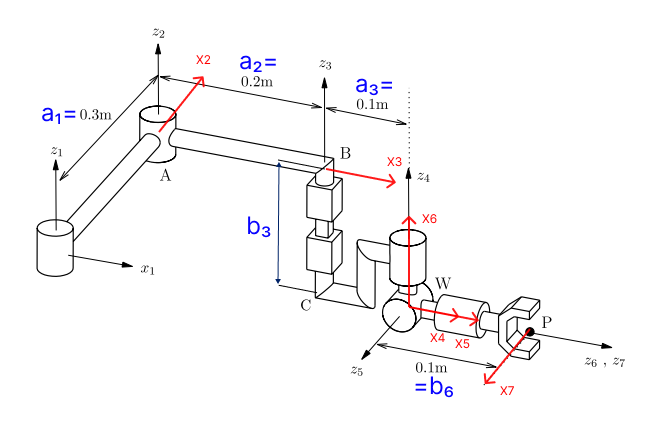
\includegraphics[width=0.4\textwidth]{figures/prob1.png}}
    \caption{Schematic view of robot marked up with D-H vectors}
    \label{fig:prob1}
\end{figure}

\begin{table}[htbp]
    \caption{The D-H parameters of 6-DOF robot}
    \def\arraystretch{1.75}
    \begin{center}
        \begin{tabular}{|Y|Y|Y|Y|Y|}
            \hline
            $i$ & $a_i$ & $b_i$ & $\alpha_i$      & $\theta_i$ \\
            \hline
            1   & 0.3   & 0     & 0               & $\theta_1$ \\
            \hline
            2   & 0.2   & 0     & 0               & $\theta_2$ \\
            \hline
            3   & 0.1   & $b_3$ & 0               & 0          \\
            \hline
            4   & 0     & 0     & $\frac{\pi}{2}$ & $\theta_4$ \\
            \hline
            5   & 0     & 0     & $\frac{\pi}{2}$ & $\theta_5$ \\
            \hline
            6   & 0     & 0.1   & 0               & $\theta_6$ \\
            \hline
        \end{tabular}
    \end{center}
\end{table}

\begin{small}
    \begin{align*}
         & Q_1 = \begin{bmatrix}
                     \cos \theta_1 & - 1 \sin \theta_1 & 0 \\
                     \sin \theta_1 & 1 \cos \theta_1   & 0 \\
                     0             & 0                 & 1
                 \end{bmatrix} ,
         & Q_2 = \begin{bmatrix}
                     \cos \theta_2 & - 1 \sin \theta_2 & 0 \\
                     \sin \theta_2 & 1 \cos \theta_2   & 0 \\
                     0             & 0                 & 1
                 \end{bmatrix} , \\
         & Q_3 = \begin{bmatrix}
                     1 & 0 & 0 \\
                     0 & 1 & 0 \\
                     0 & 0 & 1
                 \end{bmatrix} = \emph{I}
         & Q_4 = \begin{bmatrix}
                     \cos \theta_4 & 0 & \sin \theta_4     \\
                     \sin \theta_4 & 0 & - 1 \cos \theta_4 \\
                     0             & 1 & 0
                 \end{bmatrix} , \\
         & Q_5 = \begin{bmatrix}
                     \cos \theta_5 & 0 & \sin \theta_5     \\
                     \sin \theta_5 & 0 & - 1 \cos \theta_5 \\
                     0             & 1 & 0
                 \end{bmatrix} ,
         & Q_6 = \begin{bmatrix}
                     \cos \theta_6 & - 1 \sin \theta_6 & 0 \\
                     \sin \theta_6 & 1 \cos \theta_6   & 0 \\
                     0             & 0                 & 1
                 \end{bmatrix} ; \\
        % -------------------------
         &                                          &  \\
        % -------------------------
         & \vec{\mathbf{a_1}} =
        \begin{bmatrix}
            0.3\cos\theta_1 \\
            0.3\sin\theta_1 \\
            0
        \end{bmatrix} ,
         & \vec{\mathbf{a_2}} =
        \begin{bmatrix}
            0.2 \cos \theta_2 \\
            0.2 \sin \theta_2 \\
            0
        \end{bmatrix} ,                              \\
         & \vec{\mathbf{a_3}} =
        \begin{bmatrix}
            0.1 \\
            0   \\
            b_3
        \end{bmatrix} , \quad
        \vec{\mathbf{a_4}} =
        \begin{bmatrix}
            0 \\
            0 \\
            0
        \end{bmatrix} = \vec{\mathit{O}} ,
         & \vec{\mathbf{a_5}} =
        \begin{bmatrix}
            0 \\
            0 \\
            0
        \end{bmatrix} = \vec{\mathit{O}} , \quad
        \vec{\mathbf{a_6}} =
        \begin{bmatrix}
            0 \\
            0 \\
            0.1
        \end{bmatrix} ;
    \end{align*}
\end{small}


The wrist point, annotated with ``W'', has the following coordinates:
\begin{align*}
    \vec{\mathbf{\mathit{P_W}}} = & \,\, \mathbf{a_1} + Q_1 \mathbf{a_2} + Q_1 Q_2 \mathbf{a_3} + Q_1 Q_2 Q_3 \mathbf{a_4};
    \quad \quad \xrightarrow[here]{\mathbf{a_4} = \vec{\mathit{O}}}
\end{align*}

\begin{small}
    \begin{align*}
        \vec{\mathbf{\mathit{P_W}}} = & \begin{bmatrix}
                                            0.3\cos\theta_1 \\
                                            0.3\sin\theta_1 \\
                                            0
                                        \end{bmatrix} +     \begin{bmatrix}
                                                                \cos \theta_1 & - 1 \sin \theta_1 & 0 \\
                                                                \sin \theta_1 & 1 \cos \theta_1   & 0 \\
                                                                0             & 0                 & 1
                                                            \end{bmatrix}     \begin{bmatrix}
                                                                                  0.2 \cos \theta_2 \\
                                                                                  0.2 \sin \theta_2 \\
                                                                                  0
                                                                              \end{bmatrix} +                \\
                                      & \begin{bmatrix}
                                            \cos \theta_1 & - 1 \sin \theta_1 & 0 \\
                                            \sin \theta_1 & 1 \cos \theta_1   & 0 \\
                                            0             & 0                 & 1
                                        \end{bmatrix} \begin{bmatrix}
                                                          \cos \theta_2 & - 1 \sin \theta_2 & 0 \\
                                                          \sin \theta_2 & 1 \cos \theta_2   & 0 \\
                                                          0             & 0                 & 1
                                                      \end{bmatrix}     \begin{bmatrix}
                                                                            0.1 \\
                                                                            0   \\
                                                                            b_3
                                                                        \end{bmatrix}                      \\
        =                             & \begin{bmatrix}
                                            0.3\cos \left(\theta_1\right) + 0.2\cos \left(\theta_1 + \theta_2\right) \\
                                            0.3\sin \left(\theta_1\right) + 0.2\sin \left(\theta_1 + \theta_2\right) \\
                                            0
                                        \end{bmatrix}
        + \begin{bmatrix}
              0.1\cos \left(\theta_1 + \theta_2\right) \\
              0.1\sin \left(\theta_1 + \theta_2\right) \\
              b_3
          \end{bmatrix}                                                               \\
        \vec{\mathbf{\mathit{P_W}}} = & \begin{bmatrix}
                                            0.3\cos \left(\theta_1\right) + 0.3\cos \left(\theta_1 + \theta_2\right) \\
                                            0.3\sin \left(\theta_1\right) + 0.3\sin \left(\theta_1 + \theta_2\right) \\
                                            b_3
                                        \end{bmatrix} \quad \quad \quad \quad \quad \longleftarrow
    \end{align*}
\end{small}


\section{Problem 2:  Motoman-EA1400N Welding Robot}
Using the datasheet \cite{b3} of the specified welding robot, its D-H parameters can be listed in Table~\ref{tab:prob2} and shown in Figure~\ref{fig:prob2}.

\begin{table}[htbp]
    \caption{The D-H parameters of Motoman-EA1400N Welding robot}
    \label{tab:prob2}
    \def\arraystretch{1.75}
    \begin{center}
        \begin{tabular}{|Y|Y|Y|Y|Y|}
            \hline
            $i$ & $a_i$ & $b_i$ & $\alpha_i$ & $\theta_i$ \\
            \hline
            1   & 150   & 450   & $\pi/2$    & $\theta_1$ \\
            \hline
            2   & 570   & 0     & $\pi$      & $\theta_2$ \\
            \hline
            3   & 200   & 0     & $\pi/2$    & $\theta_3$ \\
            \hline
            4   & 0     & 640   & $\pi/2$    & $\theta_4$ \\
            \hline
            5   & 30    & 0     & $\pi/2$    & $\theta_5$ \\
            \hline
            6   & 0     & 200   & 0          & $\theta_6$ \\
            \hline
        \end{tabular}
    \end{center}
\end{table}

\begin{figure}[htbp]
    \centerline{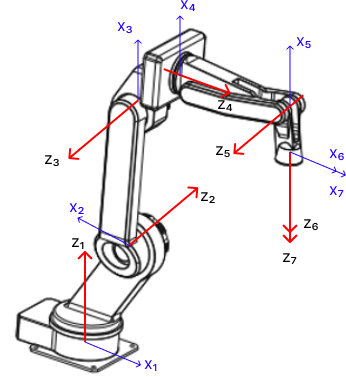
\includegraphics[width=0.4\textwidth]{figures/prob2.png}}
    \caption{Schematic view of welding robot marked up with D-H vectors}
    \label{fig:prob2}
\end{figure}

As it can be seen from both Figure~\ref{fig:prob2} and Table~\ref{tab:prob2}, there is a small $(30 mm)$ offset between axes $Z_5$ and $Z_6$. Therefor, the robot has no wrist point and thus, is \underline{not} \textit{decoupled}.

Using equations \ref{eq:Q} and \ref{eq:a}, we can find $Q_i$s and $\mathbf{a}_i$s and form the FKP equations utilizing their results.

\begin{small}
    \begin{align*}
         & Q_1 = \begin{bmatrix}
                     \cos \theta_1 & 0 & \sin \theta_1   \\
                     \sin \theta_1 & 0 & - \cos \theta_1 \\
                     0             & 1 & 0
                 \end{bmatrix} , \quad
        Q_2 = \begin{bmatrix}
                  \cos \theta_2 & \sin \theta_2   & 0  \\
                  \sin \theta_2 & - \cos \theta_2 & 0  \\
                  0             & 0               & -1
              \end{bmatrix} ,   \\
         & Q_3 = \begin{bmatrix}
                     \cos \theta_3 & 0 & \sin \theta_3   \\
                     \sin \theta_3 & 0 & - \cos \theta_3 \\
                     0             & 1 & 0
                 \end{bmatrix}, \quad
        Q_4 = \begin{bmatrix}
                  \cos \theta_4 & 0 & \sin \theta_4   \\
                  \sin \theta_4 & 0 & - \cos \theta_4 \\
                  0             & 1 & 0
              \end{bmatrix} ,    \\
         & Q_5 = \begin{bmatrix}
                     \cos \theta_5 & 0 & \sin \theta_5   \\
                     \sin \theta_5 & 0 & - \cos \theta_5 \\
                     0             & 1 & 0
                 \end{bmatrix} , \quad
        Q_6 = \begin{bmatrix}
                  \cos \theta_6 & - \sin \theta_6 & 0 \\
                  \sin \theta_6 & \cos \theta_6   & 0 \\
                  0             & 0               & 1
              \end{bmatrix} ;    \\
        % -------------------------
         &                                        &  \\
        % -------------------------
         & \vec{\mathbf{a_1}} =
        \begin{bmatrix}
            150 \cos\theta_1 \\
            150 \sin\theta_1 \\
            450
        \end{bmatrix} , \quad
        \vec{\mathbf{a_2}} =
        \begin{bmatrix}
            570 \cos \theta_2 \\
            570 \sin \theta_2 \\
            0
        \end{bmatrix} , \quad
        \vec{\mathbf{a_3}} =
        \begin{bmatrix}
            200 \cos \theta_3 \\
            200 \sin \theta_3 \\
            0
        \end{bmatrix} ,                            \\
         & \vec{\mathbf{a_4}} =
        \begin{bmatrix}
            0 \\
            0 \\
            640
        \end{bmatrix} , \quad \quad \quad \quad
        \vec{\mathbf{a_5}} =
        \begin{bmatrix}
            30 \cos \theta_5 \\
            30 \sin \theta_5 \\
            0
        \end{bmatrix} , \quad
        \vec{\mathbf{a_6}} =
        \begin{bmatrix}
            0 \\
            0 \\
            200
        \end{bmatrix} ;
    \end{align*}
\end{small}


The \textit{end-effector} point, has the following coordinates based on a more complete format of equation \ref{eq:P}, which is mentioned below in equation \ref{eq:C}.
\begin{align}
    \vec{\mathbf{\mathit{P_{EE}}}} = & \,\, \mathbf{a_1} + Q_1 \mathbf{a_2} + Q_1 Q_2 \mathbf{a_3} + Q_1 Q_2 Q_3 \mathbf{a_4} + \label{eq:C} \\
                                     & Q_1 Q_2 Q_3 Q_4 \mathbf{a_5} + Q_1 Q_2 Q_3 Q_4 Q_5 \mathbf{a_6} \nonumber
\end{align}

Thus, by substituting values and multiplying required matrices in \textbf{Python}\footnote{\, This code is appended in the end of this report and accompanies its file as well.}, we can have the result as below\footnote{\, The terms notated as \textit{t1}, \textit{t2}, \dots, \textit{6} in the upcoming lines, refer to $\theta_1$, $\theta_2$, \dots, $\theta_6$, correspondingly.}.
\begin{align*}
    \vec{\mathbf{\mathit{P_{EE}}}} = \begin{bmatrix}
                                         X \\
                                         Y \\
                                         Z
                                     \end{bmatrix}
    \quad\quad\quad\quad \text{while: }
\end{align*}

% \begin{footnotesize}
%     $\mathbf{X} = $ \texttt{200*(-sin(t1)*sin(t4) + cos(t1)*cos(t4)*cos(t2 - t3))*sin(t5) - 30*(sin(t1)*sin(t4) - cos(t1)*cos(t4)*cos(t2 - t3))*cos(t5) + 10*(-64*sin(t2 - t3) + 57*cos(t2) + 20*cos(t2 - t3) + 15)*cos(t1) - 30*sin(t5)*sin(t2 - t3)*cos(t1) + 200*sin(t2 - t3)*cos(t1)*cos(t5)} \\
%     $\mathbf{Y} = $ \texttt{200*(sin(t1)*cos(t4)*cos(t2 - t3) + sin(t4)*cos(t1))*sin(t5) + 30*(sin(t1)*cos(t4)*cos(t2 - t3) + sin(t4)*cos(t1))*cos(t5) + 10*(-64*sin(t2 - t3) + 57*cos(t2) + 20*cos(t2 - t3) + 15)*sin(t1) - 30*sin(t1)*sin(t5)*sin(t2 - t3) + 200*sin(t1)*sin(t2 - t3)*cos(t5)} \\
%     $\mathbf{Z} = $ \texttt{570*sin(t2) + 200*sin(t5)*sin(t2 - t3)*cos(t4) + 30*sin(t5)*cos(t2 - t3) + 30*sin(t2 - t3)*cos(t4)*cos(t5) + 200*sin(t2 - t3) - 200*cos(t5)*cos(t2 - t3) + 640*cos(t2 - t3) + 450}
% \end{footnotesize}

\begin{small}
    $\mathbf{X} = 200  (-\sin(t1)  \sin(t4) + \cos(t1)  \cos(t4)  \cos(t2 - t3))  \sin(t5) - 30  (\sin(t1)  \sin(t4) - \cos(t1)  \cos(t4)  \cos(t2 - t3))  \cos(t5) + 10  (-64  \sin(t2 - t3) + 57  \cos(t2) + 20  \cos(t2 - t3) + 15)  \cos(t1) - 30  \sin(t5)  \sin(t2 - t3)  \cos(t1) + 200  \sin(t2 - t3)  \cos(t1)  \cos(t5)$ \\

    $\mathbf{Y} = 200  (\sin(t1)  \cos(t4)  \cos(t2 - t3) + \sin(t4)  \cos(t1))  \sin(t5) + 30  (\sin(t1)  \cos(t4)  \cos(t2 - t3) + \sin(t4)  \cos(t1))  \cos(t5) + 10  (-64  \sin(t2 - t3) + 57  \cos(t2) + 20  \cos(t2 - t3) + 15)  \sin(t1) - 30  \sin(t1)  \sin(t5)  \sin(t2 - t3) + 200  \sin(t1)  \sin(t2 - t3)  \cos(t5)$ \\

    $\mathbf{Z} = 570  \sin(t2) + 200  \sin(t5)  \sin(t2 - t3)  \cos(t4) + 30  \sin(t5)  \cos(t2 - t3) + 30  \sin(t2 - t3)  \cos(t4)  \cos(t5) + 200  \sin(t2 - t3) - 200  \cos(t5)  \cos(t2 - t3) + 640  \cos(t2 - t3) + 450$
\end{small}

\vspace{30px}
\section{Problem 4: IKP}
Same as previous problems, we form the D-H table after highlighting its parameters in Figure~\ref{fig:prob4}.

\begin{figure}[htbp]
    \centerline{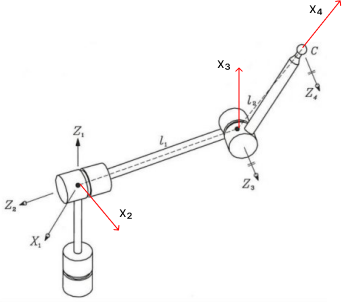
\includegraphics[width=0.4\textwidth]{figures/prob4.png}}
    \caption{Schematic view of robot marked up with D-H vectors}
    \label{fig:prob4}
\end{figure}

\begin{table}[htbp]
    \caption{The D-H parameters of 3-DOF robot}
    \def\arraystretch{1.75}
    \begin{center}
        \begin{tabular}{|Y|Y|Y|Y|Y|}
            \hline
            $i$ & $a_i$ & $b_i$  & $\alpha_i$ & $\theta_i$ \\
            \hline
            1   & 0     & 0      & $\pi / 2$  & $\theta_1$ \\
            \hline
            2   & 0     & $-l_1$ & $\pi / 2$  & $\theta_2$ \\
            \hline
            3   & $l_2$ & 0      & 0          & $\theta_3$ \\
            \hline
        \end{tabular}
    \end{center}
\end{table}

Using equations \ref{eq:Q} and \ref{eq:a}, we can find $Q_i$s and $\mathbf{a}_i$s and obtain the FKP problem utilizing their results.

\begin{small}
    \begin{align*}
         & \left[Q_1\right] = \begin{bmatrix}
                                  \cos \theta_1 & 0 & \sin \theta_1   \\
                                  \sin \theta_1 & 0 & - \cos \theta_1 \\
                                  0             & 1 & 0
                              \end{bmatrix} \quad
        \left[Q_2\right] = \begin{bmatrix}
                               \cos \theta_2 & 0 & \sin \theta_2   \\
                               \sin \theta_2 & 0 & - \cos \theta_2 \\
                               0             & 1 & 0
                           \end{bmatrix}    \\
         & \left[Q_3\right] = \begin{bmatrix}
                                  \cos \theta_3 & - \sin \theta_3 & 0 \\
                                  \sin \theta_3 & \cos \theta_3   & 0 \\
                                  0             & 0               & 1
                              \end{bmatrix} \\
        % -------------------------
         &                                        &               \\
        % -------------------------
         & \vec{\mathbf{a_1}} =
        \begin{bmatrix}
            0 \\
            0 \\
            0
        \end{bmatrix} \quad\quad\quad
        \vec{\mathbf{a_2}} =
        \begin{bmatrix}
            0 \\
            0 \\
            -l_1
        \end{bmatrix} \quad\quad\quad
        \vec{\mathbf{a_3}} =
        \begin{bmatrix}
            l_2 \cos \theta_3 \\
            l_2 \sin \theta_3 \\
            0
        \end{bmatrix}
    \end{align*}
\end{small}

By generalizing the equation \ref{eq:C} and using it for a 3-DOF robot, the same as what we have in this problem, we get the \textit{end-effector }position like:
\begin{small}
    \begin{align*}
        \vec{\mathbf{\mathit{P_{EE}}}} = & \,\, \mathbf{a_1} + Q_1 \mathbf{a_2} + Q_1 Q_2 \mathbf{a_3} \quad \quad \quad \quad \xrightarrow[here]{\mathbf{a_1} = \vec{\mathit{O}}} \\
        \vec{\mathbf{\mathit{P_c}}} =    & \begin{bmatrix}
                                               x_c \\
                                               y_c \\
                                               z_c
                                           \end{bmatrix}
        = \begin{bmatrix}
              \cos \theta_1 & 0 & \sin \theta_1   \\
              \sin \theta_1 & 0 & - \cos \theta_1 \\
              0             & 1 & 0
          \end{bmatrix} \begin{bmatrix}
                            0 \\
                            0 \\
                            -l_1
                        \end{bmatrix} +                                                                                                                                      \\
                                         & \begin{bmatrix}
                                               \cos \theta_1 & 0 & \sin \theta_1   \\
                                               \sin \theta_1 & 0 & - \cos \theta_1 \\
                                               0             & 1 & 0
                                           \end{bmatrix} \begin{bmatrix}
                                                             \cos \theta_2 & 0 & \sin \theta_2   \\
                                                             \sin \theta_2 & 0 & - \cos \theta_2 \\
                                                             0             & 1 & 0
                                                         \end{bmatrix} \begin{bmatrix}
                                                                           l_2 \cos \theta_3 \\
                                                                           l_2 \sin \theta_3 \\
                                                                           0
                                                                       \end{bmatrix}                                                                                       \\
        \vec{\mathbf{\mathit{P_c}}} =    & \begin{bmatrix}
                                               -l_1 \sin\theta_1 + l_2 (\cos\theta_1 \cos\theta_2 \cos\theta_3 + \sin\theta_1 \sin\theta_3) \\
                                               l_1 \cos\theta_1 + l_2 (\sin\theta_1 \cos\theta_2 \cos\theta_3 - \cos\theta_1 \sin\theta_3)  \\
                                               l_2 \sin\theta_2 \cos\theta_3
                                           \end{bmatrix}
    \end{align*}
\end{small}

In a special case where $\theta_1 = \theta_2 = \theta_3 = 90^\circ$, this term will be simplified to:
$$
    \vec{\mathbf{\mathit{P_c}}} = \begin{bmatrix}
        l_2 - l_1 \\
        0         \\
        0
    \end{bmatrix}
$$

Now we form the IKP problem's equations:
\begin{align}
     & x = -l_1 \sin\theta_1 + l_2 (\cos\theta_1 \cos\theta_2 \cos\theta_3 + \sin\theta_1 \sin\theta_2) \label{eq:one} \\
     & y = l_1 \cos\theta_1 + l_2 (\sin\theta_1 \cos\theta_2 \cos\theta_3 - \cos\theta_1 \sin\theta_2)  \label{eq:two} \\
     & z = l_2 \sin\theta_2 \cos\theta_3 \label{eq:four}
\end{align}
By dividing equations \ref{eq:one} by \ref{eq:two} and manipulating algebraic terms, we get a simplified result:
\begin{align}
     & x \sin \theta_1 = l_2 \sin \theta_3 + y \cos \theta_1 - l_1 \label{eq:three}
\end{align}
We also have:
\begin{align}
     & \sin ^2 \theta_2 + \cos ^2 \theta_2 = 1 \label{eq:five}                                                                                                                           \\
     & \xRightarrow{\ref{eq:one}} cos \theta_2 = \frac{x - l_2 \sin \theta_1 \sin \theta_3 + l_1 \sin \theta_1}{l_2 \cos \theta_3 \cos \theta_1} \label{eq:six}                          \\
     & \xRightarrow{\ref{eq:four}, \, \ref{eq:three}, \, \ref{eq:five}, \, \ref{eq:six}} z^2 + x^2 \cos ^2 \theta_1 + y^2 \sin ^2 \theta_1 - 2 x y \sin \theta_1 \cos \theta_1 \nonumber \\
     & \quad \quad \quad \quad = l_2 ^2 \cos ^2 \theta_3 \label{eq:seven}                                                                                                                \\
     & \xRightarrow{\ref{eq:three}} l_2 ^2 \sin ^2 \theta_3 = l_1 ^2 + x^2 \sin ^2 \theta_1 + y^2 \cos ^2 \theta_1 + 2 x l_1 \sin \theta_1 \nonumber                                     \\
     & \quad \quad \quad \quad \quad \quad \,\, - 2 y l_1 \cos \theta_1 - 2 x y \sin \theta_1 \cos \theta_1 \label{eq:eight}
\end{align}
Introducing $\sin \theta_1 = \frac{2 t}{1 + t^2}$ and $\cos \theta_1 = \frac{1 - t^2}{1 + t^2}$ while $t = \tan (\frac{\theta_1}{2})$, we'll get:
\begin{align}
     & \xRightarrow{\ref{eq:seven}, \ref{eq:eight}} x^2 + y^2 + z^2 - 4 x y (\frac{2 t}{1 + t^2}) (\frac{1 - t^2}{1 + t^2}) - \nonumber \\
     & \quad \quad \quad 2 l_1 (\frac{2 t x}{1 + t^2} - \frac{(1 - t^2) y}{1 + t^2}) + l_1 ^2 = l_3 ^2                                  \\
     & \xRightarrow{\text{simplifying}} \mathbf{A t^4 + B t^3 + C t^2 + D t + E = 0}
\end{align}
While,
\begin{align*}
     & \mathbf{A} = x^2 + y^2 + z^2 + l_1 ^2 + l_2 ^2 + 2 l_1 y \\
     & \mathbf{B} = 8 x y + 4 l_1                               \\
     & \mathbf{C} = x^2 + y^2 + z^2 + l_1 ^2 + l_2 ^2           \\
     & \mathbf{D} = 8 x y - 4 l_1                               \\
     & \mathbf{E} = x^2 + y^2 + z^2 + l_1 ^2 + l_2 ^2 - 2 l_1 y
\end{align*}
Solving this \textit{Quartic equation} gives, optimistically, 4 answers for $t$. With these 4 answers, we can calculate four pairs of $\sin \theta_1$ and $\cos \theta_1$ using the definition of $t$ mentioned before. Putting each of these 4 pairs into $\theta_1 = \arctan2(\sin \theta_1, \cos \theta_1)$, gives 4 answers for $\theta_1$ corresponding to each $t$. Afterwards, equation \ref{eq:three} gives:
$$
    \theta_3 = \arcsin \left(\frac{x \sin \theta_1 - y \cos \theta_1 - l_1}{l_2}\right)
$$
This will give 2 answers for $\theta_3$ for each $\theta_1$ we substitute in it. So, using the derived equations, we'll have an \underline{overall of 8 pairs of answers} for $\theta_1$ and $\theta_3$ which were asked in this problem.

\begin{large}
    \begin{align*}
         & answers \longrightarrow \begin{cases}
                                       \theta_1 ^1 & \longrightarrow \begin{cases}
                                              \theta_3 ^1 \\[10pt]
                                              \theta_3 ^2
                                          \end{cases} \\[30pt]
                                       \theta_1 ^2 & \longrightarrow \begin{cases}
                                              \theta_3 ^3 \\[10pt]
                                              \theta_3 ^4
                                          \end{cases} \\[30pt]
                                       \theta_1 ^3 & \longrightarrow \begin{cases}
                                              \theta_3 ^5 \\[10pt]
                                              \theta_3 ^6
                                          \end{cases} \\[30pt]
                                       \theta_1 ^4 & \longrightarrow \begin{cases}
                                              \theta_3 ^7 \\[10pt]
                                              \theta_3 ^8
                                          \end{cases} \\
                                   \end{cases}
    \end{align*}
\end{large}

\vspace{30px}

\section{Conclusion}
\textbf{
    In conclusion, this report has provided a comprehensive overview of several important concepts in robotics such as D-H parameters, FKP, IKP and wrist robots. We tackled forward and inverse kinematics for various serial robots. Leveraging conformal geometric algebra, we derived elegant formulations for both problems. Our approach excelled in solving the inverse kinematics for manipulators with a spherical wrist. We adhered to the widely used Denavit-Hartenberg (D-H) convention, which standardized coordinate frames for spatial linkages. The D-H parameters—link length, link twist, and other dimensions—characterized our serial robots' kinematics. Moving forward, this knowledge will serve as a solid foundation for further exploration and experimentation of ours, in robotics field.
}
\vspace{20px}

\begin{thebibliography}{00}
    \bibitem{b1} J. Angeles, ``Fundamentals of Robotic Mechanical Systems'', Theory, Methods, and Algorithms, 4th edition, Springer.

    \bibitem{b2} J. J. Craig, ``Introduction to Robotics'', 3d edition, Pearson Education, Inc.

    \bibitem{b3} T.I.E industrial, ``Motoman EA1400N'', ROBOTS.com, \url{https://www.robots.com/industrial-robots/motoman-ea1400n}

    \bibitem{b4} N. Kofinas, E. Orfanoudakis, M. G. Lagoudakis, ``Complete Analytical Forward and Inverse Kinematics for the NAO Humanoid Robot''. J Intell Robot Syst 77, (2015). [Online]. Available: \url{https://doi.org/10.1007/s10846-013-0015-4}

    \bibitem{b5} M. Ceccarelli, M. Russo, (2020). ``Parallel Architectures for Humanoid Robots''. Robotics, 9(4). [Online]. Available: \url{https://doi.org/10.3390/robotics9040075}
\end{thebibliography}

% ----------------------------------------------------------------------------
\section{Appendix}
\subsection{Python code for problem 2}
\begin{lstlisting}[language=Python]
from sympy import *

t1, t2, t3, t4, t5, t6 = symbols('t1, t2, t3, t4, t5, t6')

a = [None for i in range(6)]
Q = [None for i in range(7)]

Q[0] = Matrix([
    [cos(t1), 0, sin(t1)],
    [sin(t1), 0, -cos(t1)],
    [0, 1, 0]
])

Q[1] = Matrix([
    [cos(t2), sin(t2), 0],
    [sin(t2), -cos(t2), 0],
    [0, 0, -1]
])

Q[2] = Matrix([
    [cos(t3), 0, sin(t3)],
    [sin(t3), 0, -cos(t3)],
    [0, 1, 0]
])

Q[3] = Matrix([
    [cos(t4), 0, sin(t4)],
    [sin(t4), 0, -cos(t4)],
    [0, 1, 0]
])

Q[4] = Matrix([
    [cos(t5), 0, sin(t5)],
    [sin(t5), 0, -cos(t5)],
    [0, 1, 0]
])

Q[5] = Matrix([
    [cos(t6), -sin(t6), 0],
    [sin(t6), cos(t6), 0],
    [0, 0, 1]
])

Q[6] = eye(3, 3)

a[0] = 150*Matrix([
    [cos(t1)],
    [sin(t1)],
    [3]
])

a[1] = 570*Matrix([
    [cos(t2)],
    [sin(t2)],
    [0]
])

a[2] = 200*Matrix([
    [cos(t3)],
    [sin(t3)],
    [0]
])

a[3] = 640*Matrix([
    [0],
    [0],
    [1]
])

a[4] = 30*Matrix([
    [cos(t5)],
    [sin(t5)],
    [0]
])

a[5] = 200*Matrix([
    [0],
    [0],
    [1]
])

P = zeros(3, 1)
ans = eye(3, 3)
for i in range(6):
    ans = ans@Q[i-1]
    P += ans@a[i]
    P = simplify(P)

pprint(P)
print()
print(matrix2numpy(P))
print()
\end{lstlisting}
% ----------------------------------------------------------------------------

\end{document}
